\section{Exploring Stokes paradox*}
\label{sec:creeping_cylinder}

Stokes paradox is very soon encountered. Our task is to solve the
bi-Laplace equation, Eq. \ref{eq:bi-laplacian}, for a 2D case, in
which the vector potential $\bfA$ only has a $z$ component, equal to
the stream function $\psi$. Then,
\[
  \nabla^4 \psi = 0 ,
\]
from which $u=\nabla\times\psi$. Finally, the pressure field is
obtained from Stokes equation, \ref{eq:Stokes}:
$\nabla p = \mu \nabla^2 \bfu$.

In polar coordinates,
\begin{equation}
  \label{eq:Lapl_in_polar}
  \nabla^2 \psi =
  {1 \over  r}{\partial \over \partial  r}\left(
    r {\partial f \over \partial  r}\right)
  + {1 \over  r^2}{\partial^2 f \over \partial \theta^2} .
\end{equation}

Trying a function $\psi = r^\alpha \sin\theta$, we find that
\begin{equation*}
  \nabla^2   r^\alpha \sin\theta  =
  r^{\alpha-2} \sin\theta \left( \alpha^2 -1  \right) .
\end{equation*}

This means the only two possibilities are $\alpha=\pm 1$. Indeed, the
potential solution for the flow past a cylinder was built from these
two solutions (see e.g. Eq \ref{eq:pot_phi_guess}).

The bi-Laplacian is then
\begin{equation*}
  \nabla^4   r^\alpha \sin\theta  =
  r^{\alpha-4} \sin\theta
  \left( \alpha^2 -1  \right)
  \left( (\alpha-2)^2 -1  \right) .
\end{equation*}
The ``new'' possible exponents are now $\alpha=3$ and $\alpha=1$. The
first one is of no use, since it leads to the wrong behavior away from
the cylinder. The second one is not new at all! We are therefore stuck
with the same functional set as for potential flow. This is, in a
nutshell, the paradox.

This means that the only sensible solution is the potential one, which
of course features free-slip boundary conditions on the surface of the
cylinder. The resulting pressure field will be constant, since
$\nabla p = \mu \nabla^2 \bfu$, but these two functions have null
Laplacian. This field would, however, have a non-zero shear stress on
the cylinder, as we will discuss below.

The traditional way of dealing with this situation is to reject Stokes
equation \ref{eq:Stokes} as an adecuate model of the situation. The
perturbation in the velocity field is so great that any Reynolds
number is bound to be not so small after that --- in the sense that
the relevant length in Re=$\rho L u_0 /\mu$ is surely not the radius
of the cylinder, but a much larger value.

We present here an exploration of another way past this issue, which
could be interesting, but is -- we caution the reader -- fraught with
tricks.

Let us consider the next term, $\psi = r^\alpha \sin (2 \theta)$. Then
\begin{align*}
  \nabla^2   r^\alpha \sin(2 \theta)  &=
                                        r^{\alpha-2} \sin(2\theta) \left( \alpha^2 -4  \right) \\
  \nabla^4   r^\alpha \sin(2 \theta)  &=
                                        r^{\alpha-4} \sin(2\theta) \left( (\alpha-2)^2 -4  \right) .
\end{align*}
The solutions are then: $\alpha=\pm 2$ for the Laplace equation, and
$\alpha=0$ and $4$ for the bi-Laplacian. Again, the $2$ and $4$
exponents are to be rejected, but we may combine the $0$ and $-2$ ones
(remembering the latter is a solution of Laplace equation.)

Let us write
\[
  \psi =
  R u_0 \left[ \frac{r}{R} - \frac{1}{r} \right] \sin\theta -
  R w_0 \left[ 1 - \left( \frac{R}{r}\right)^2 \right] \sin( 2\theta) ,
\]
where $w_0$ is some unknown velocity.

The second term is chosen this way because the radial velocity
component is then
\begin{equation*}
  u_r= \frac{1}{r}\frac{\partial \psi}{\partial \theta} =
  u_0 \left[ 1  - \left( \frac{R}{r}\right)^2 \right] \cos\theta -
  2 w_0 \left[ \frac{R}{r} - \left( \frac{R}{r}\right)^3 \right] \cos( 2\theta) ,
\end{equation*}
which vanishes at the cylinder surface, $r=R$.

The tangential velocity is
\begin{equation*}
  u_\theta= - \frac{\partial \psi}{\partial r} =
  - u_0 \left[ 1  + \left( \frac{R}{r}\right)^2 \right] \sin\theta +
  2 w_0 \left( \frac{R}{r}\right)^3 \sin( 2\theta) .
\end{equation*}

At the surface, then
\begin{equation*}
  u_\theta(R) =
  - 2 u_0 \sin\theta + 2 w_0 \sin( 2\theta) .
\end{equation*}

The value of $w_0$ therefore determines at which points of the
cylinder is the velocity null (these are actually lines, in the $z$
direction). Common sense dictates these points occur at angles between
$0$ and $\pi/2$. This means $w_0$ should be positive, and comparable
to $u_0$. The simplest choice will be taken here, $w_0 = u_0$,
resulting in angles $\theta=\pm \pi/3$, at which the velocity is zero.
The resulting streamlines are plotted in
\ref{fig:creeping_flow_past_cyl}. The figure is very pleasing, which
is our original motivation in exploring this matter. The streamlines
as we move with the cylinder,
Fig. \ref{fig:creeping_flow_past_cyl_moving} are equally pleasing.

\begin{figure}
  \centering
  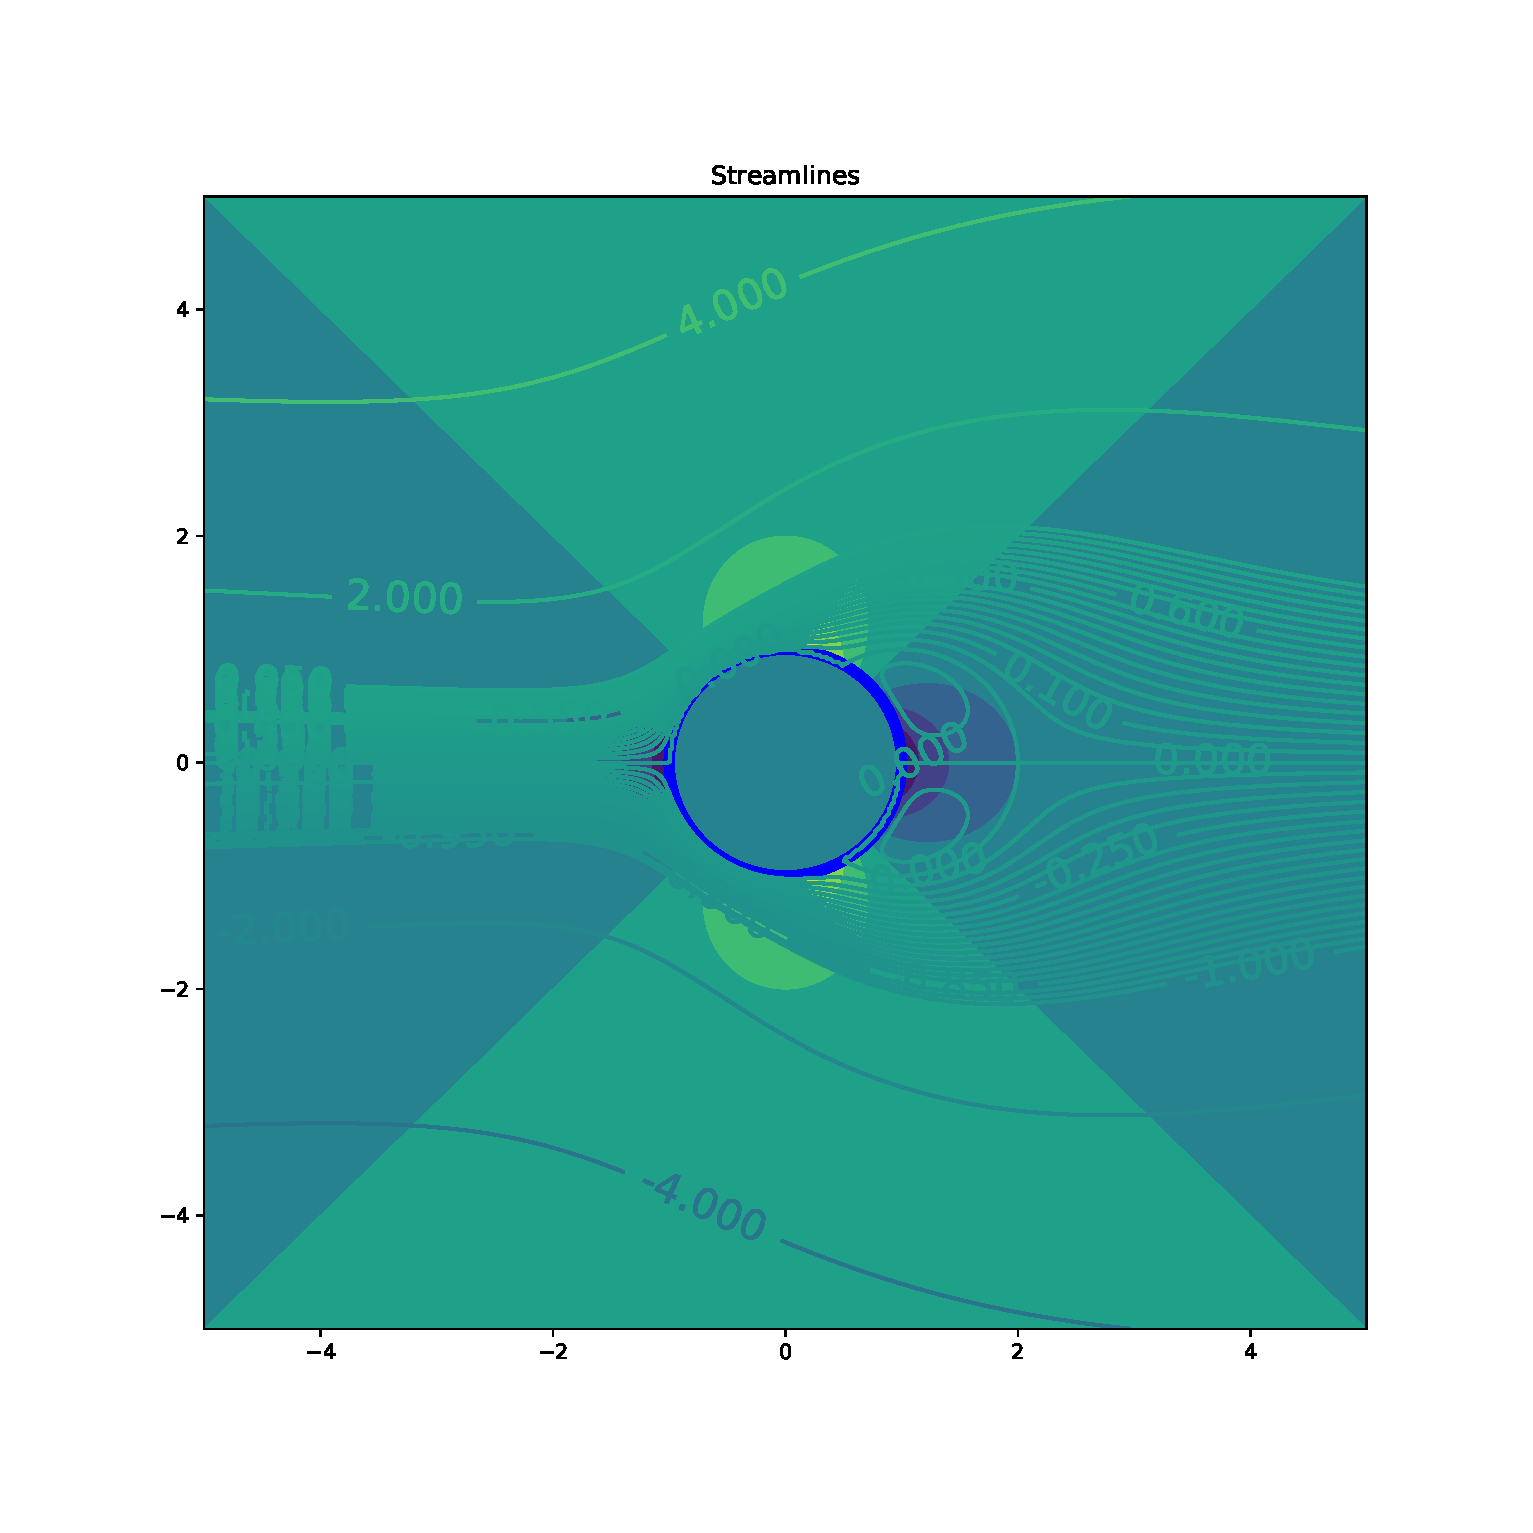
\includegraphics[width=0.8\linewidth]{figures/creeping_flow_past_cyl_slip}
  \caption{\label{fig:creeping_flow_past_cyl}}
\end{figure}


\begin{figure}
  \centering
  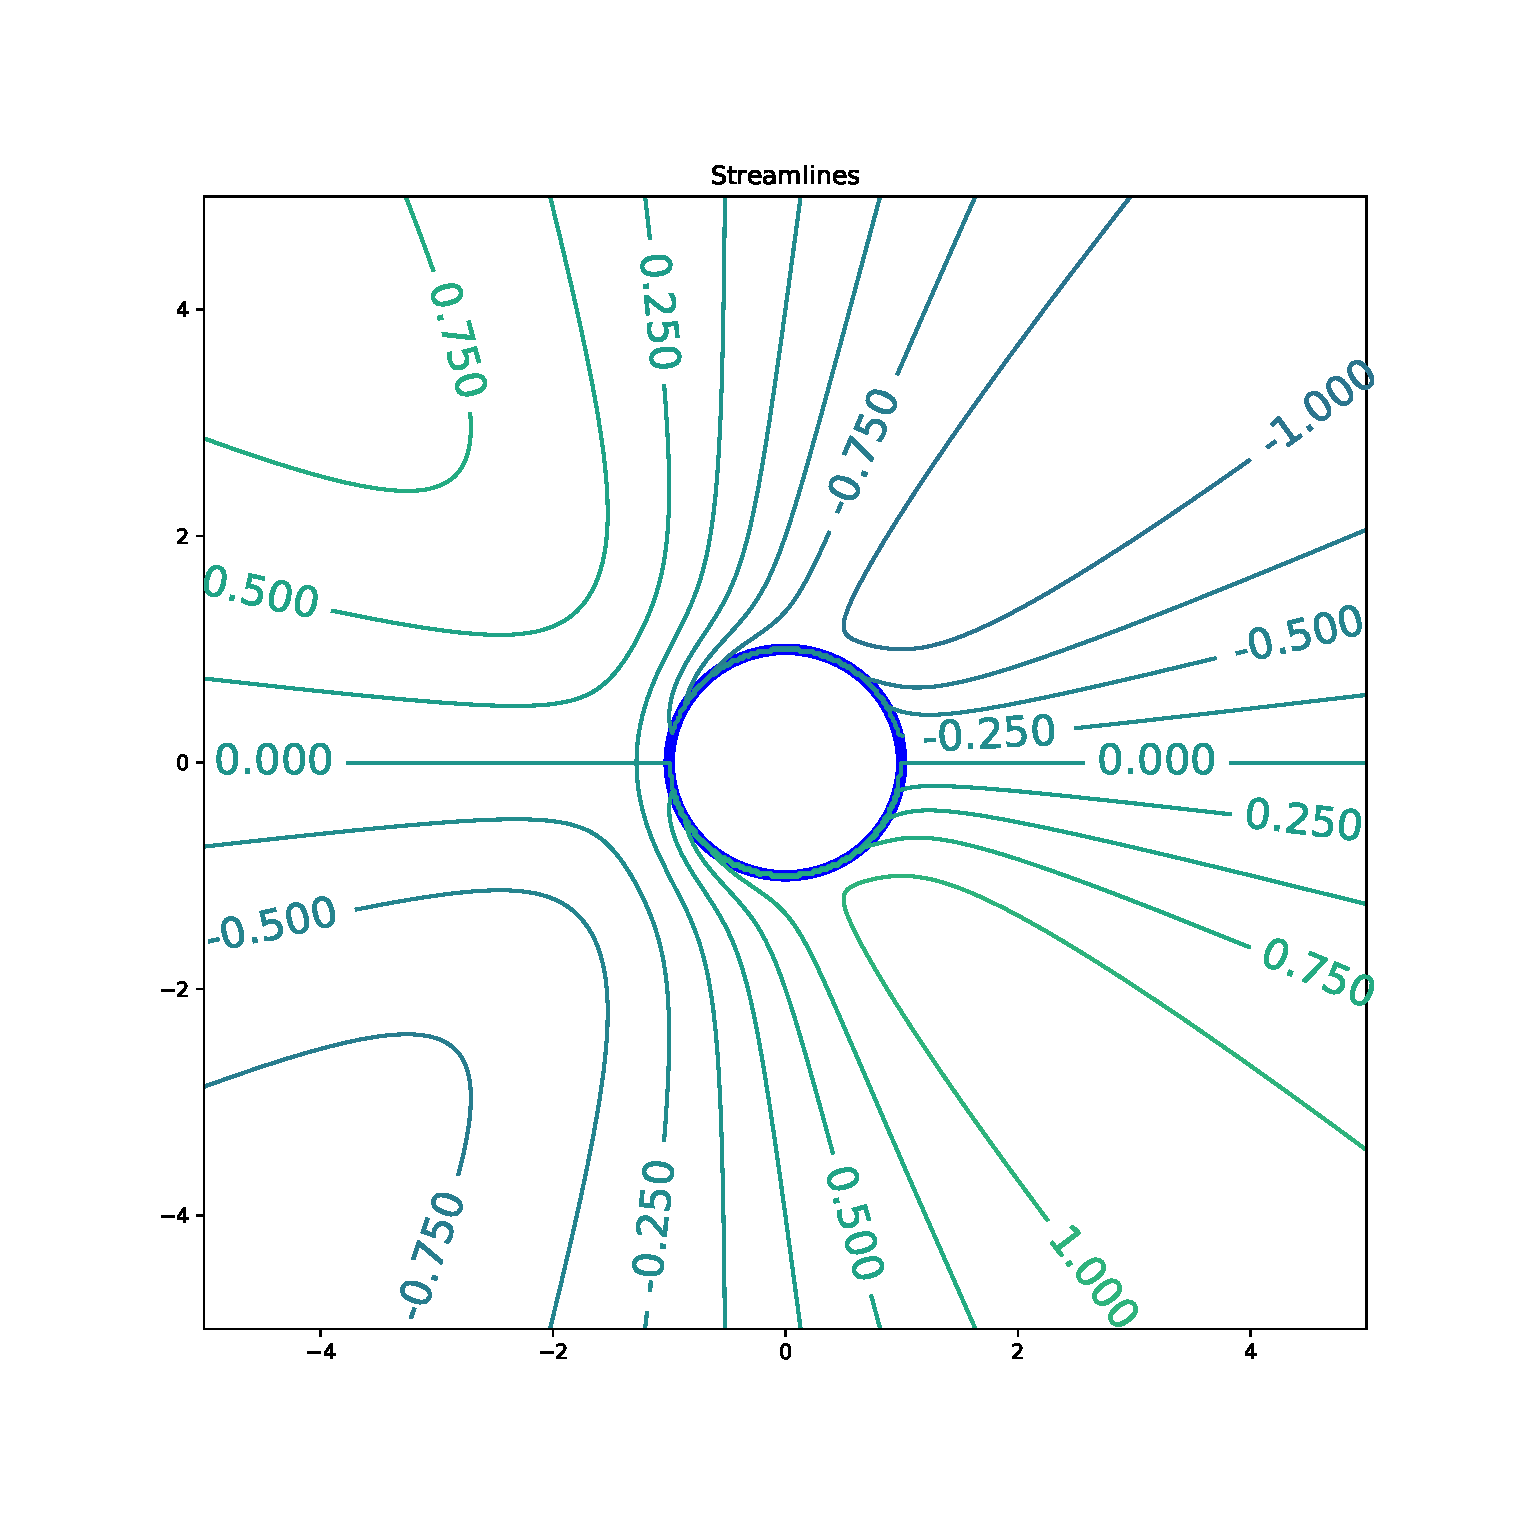
\includegraphics[width=0.8\linewidth]{figures/creeping_flow_past_cyl_slip_moving}
  \caption{\label{fig:creeping_flow_past_cyl_moving}}
\end{figure}


The resulting pressure field only has a non-trivial contribution from
the $\alpha=0$ term, since all other three are harmonic
(i.e. solutions of Laplace equation.)

The vector Laplacian is given by
\begin{align*}
(\nabla^2\bfu)_r &= \nabla^2 u_r - \frac{u_r}{r^2} - \frac{2}{r^2}
           \frac{\partial u_\theta}{\partial \theta} \\
(\nabla^2\bfu)_\theta &= \nabla^2 u_\theta - \frac{u_\theta}{r^2} + \frac{2}{r^2}
           \frac{\partial u_r}{\partial \theta} ,  
\end{align*}
with the scalar $\nabla^2$ expression as before in Eq.
\ref{eq:Lapl_in_polar}. We obtain
\begin{align*}
  (\nabla^2\bfu)_r &=   \frac{8 R u_0}{r^3} \cos(2 \theta)  \\
  (\nabla^2\bfu)_\theta &=    \frac{8 R u_0}{r^3} \sin(2 \theta)   .
\end{align*}

The pressure field is obtained from $\nabla p = \mu \nabla^2 \bfu$,
which in polar coordinates reads
\begin{align*}
  (\nabla p)_r     &=               \frac{\partial p }{  \partial r } = \mu(\nabla^2\bfu)_r  \\
  (\nabla p)_\theta &=  \frac{1}{r} \frac{\partial p }{  \partial \theta } = \mu(\nabla^2\bfu)_\theta ,
\end{align*}
whose solution is
\[
  p =
  -\frac{4 \mu u_0 R }{r^2} \cos(2\theta) =
  -\frac{4 \mu u_0}{R} \left( \frac{R }{r} \right)^2 \cos(2\theta) .
\]
In the last expression we make it clear that the pressure value is set
by $\mu u_0 / R$, and therefore the total pressure force upon the
cylinder is $D_p \sim p L R \sim \mu u_0 L$. The drag force would then
be independent of the radius, as predicted in
Eq. \ref{eq:drag_cyl_guess}. This is all consistent, if somewhat
surprising, but nevertheless moot: this pressure field, with its
$\cos(2\theta)$, has a d'Alembert's paradox! Indeed, by the same
arguments as in the classical potential solution, the net pressure
force is null. This is obvious in
Fig. \ref{fig:creeping_flow_past_cyl}, where the pressure field shows
a left-right symmetry.  Mathematically,
\begin{equation}
  \label{eq:pressure_drag_on_cyl_creeping}
  \frac{  D_p }{L} =
    R \int_0^{2\pi} d\theta   p \cos\theta  =
    4 \mu u_0 \int_0^{2\pi} d\theta  \cos\theta  \cos(2\theta)  = 0.
\end{equation}
Also, the sign of the pressure is troublesome: the low-pressure areas
are at the fore and aft of the cylinder, contrary to what may be
expected (and what is found for the potential solution,
Eq. \ref{eq:press_at_cyl_pot}.)

There is now another source of drag: shear stress on the surface. The
expression for the relevant part of the stress tensor is
\[
  \tau_{r\theta} = \mu \left(
    \frac1r
    \frac{\partial u_r}{\partial \theta} +
    r \frac{\partial }{\partial r} \left( \frac{u_\theta}{r}\right) 
  \right) 
\]
(i.e. it looks exactly as in spherical coordinates,
Eq. \ref{eq:tau_r_th}).

After some computations, at the surface we obtain
\[
  \tau_{r\theta} (R)  =  \frac{4 \mu u_0}{R} \left(
    \sin\theta - 2 \sin(2\theta) 
  \right) .
\]
The surprise is, then, that the term due to the potential solution,
$\sin\theta$, will result in a net drag force, but the new one will
not. Indeed, this force will be
\begin{equation}
  \label{eq:viscous_drag_on_cyl_creeping}
  \frac{  D_\tau }{L} =
   R \int_0^{2\pi} d\theta  (\tau_{r\theta}) (- \sin\theta)  =
  - 4 \mu u_0 \int_0^{2\pi} d\theta  \sin^2\theta  =  - 4 \pi \mu u_0 .
\end{equation}
Notice there is a minus sign due to projection on the $x$ axis from
the tangential direction, as in the shear stress on the sphere.  The
result is, in a sense, worse than the vanishing pressure force: the
drag acts in the upstream direction! Notice that the $\sin\theta$
term, which is the only one contributing, comes from the potential
solution. In this solution there are two zone, at the upper and lower
points of the cylinder, at which the velocity is quite higher than
$u_0$. This means that, in the upper part of the cylinder, the shear
force will tend to rotate the cylinder counter-clockwise, in the
positive direction, to equalize velocities. The same will happen in
the lower part, with a vanishing rotation but a non-vanishing drag in
the ``wrong'' direction.

If we nevertheless define a drag coefficient as for the sphere (with
an exposed area now given by $2RL$), this would be
\[
  C_\mathrm{inertial} = \frac{  2 |D| }{ \rho u_0^2 (2 R L) } =
  \frac{ 4 \pi \mu u_0   }{ \rho u_0^2  R L } =
  8\pi \frac{1}{\mathrm{Re}} ,
\]
with a Reynolds number defined in term of the diameter $2R$:
\[
  \mathrm{Re} = \frac{ \rho u_0 ( 2 R ) }{ \mu } .
\]

Notice that we have only employed two terms of what may be an
infinite expansion in terms $\sin(n\theta)$. In this way, by means of
Fourier analysis, we would be able to produce any tangencial velocity
we wished on the surface of the cylinder. The question is, of course,
which is the ``right'' distribution, since our main target, a null
velocity, is the one that is the one that is ruled out. For instance,
we could make the velocity null at the trailing edge of the cylinder
only.

Even if we did this, the potential would not be free of the
d'Alambert's paradox: all terms would ultimately be of the form
$\cos(n\theta)$, and the resulting drag would be zero for the same
reason as for $n=2$ in Eq. \ref{eq:pressure_drag_on_cyl_creeping}.

Moreover, the shear stress would also not change! Indeed, the new
terms in the stress tensor would be of the form $\sin(n\theta)$ ---
their contribution to the drag force would be null: in Eq.
\ref{eq:viscous_drag_on_cyl_creeping} it is clear that only $n=1$ may
contribute to this force. Since the only velocity contributing is the
potential solution, whose value is fixed by the up-stream velocity, it
cannot change.
